\chapter{Applications}
\label{chapter-applications}
\begin{ChapAbstract}
This chapter presents our applications that assist customers in e-commerce based on the methods presented, including Smart Fashion Assistant, a system for online shopping support, and Magic Mirror, an application that allows users to try on clothing items virtually in an augmented reality scenario. We present an overview of each application, followed by the details of the conducted experiments, including a pilot study to evaluate their effectiveness and user satisfaction.
\end{ChapAbstract}

\section{Magic Mirror}
\subsection{Overview}

To demonstrate the efficiency of the DM-VTON framework, we developed an Augmented Reality (AR) application that can run on a local machine named Magic Mirror. This application simulates the experience of trying on garments in front of a mirror. However, instead of real garments, our application captures the user's image via the camera, applies virtual try-on processes, and displays the results on the screen. This protects the real garments from potential damage and enables faster try-on experiences. To enhance convenience, users can easily switch between different try-on garments and backgrounds using intuitive swiping gestures.



\subsection{Implementation details}

 \begin{figure}[h!]
  \centering
  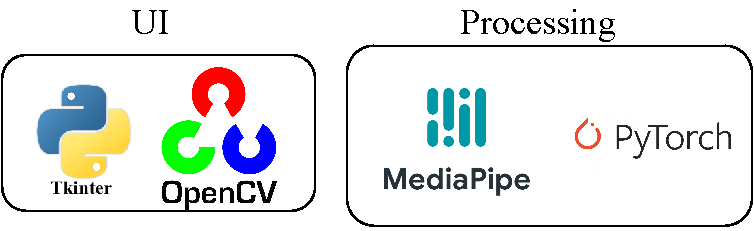
\includegraphics[width=0.7\textwidth]{content/resources/images/application/chapter5-ar-arch.pdf}
  \caption{Fundamental components of Magic Mirror}
  \label{fig:chapter5-ar-arch}
\end{figure}

\autoref{fig:chapter5-ar-arch} illustrates the fundamental architecture of Magic Mirror. We employ the Tkinter framework for the user interface display, Python's standard graphic user interface library. OpenCV is utilized to capture the user image through the camera. The captured frames are then passed to the processing components, which include MediaPipe for gesture detection and generating the background mask, as well as our DM-VTON model built on the PyTorch framework for the virtual try-on process. We deploy the application on an Acer nitro 5 AN517 laptop with an RTX 3050Ti GPU.


\subsection{Usage and Examples}
 \begin{figure}[h!]
  \centering
  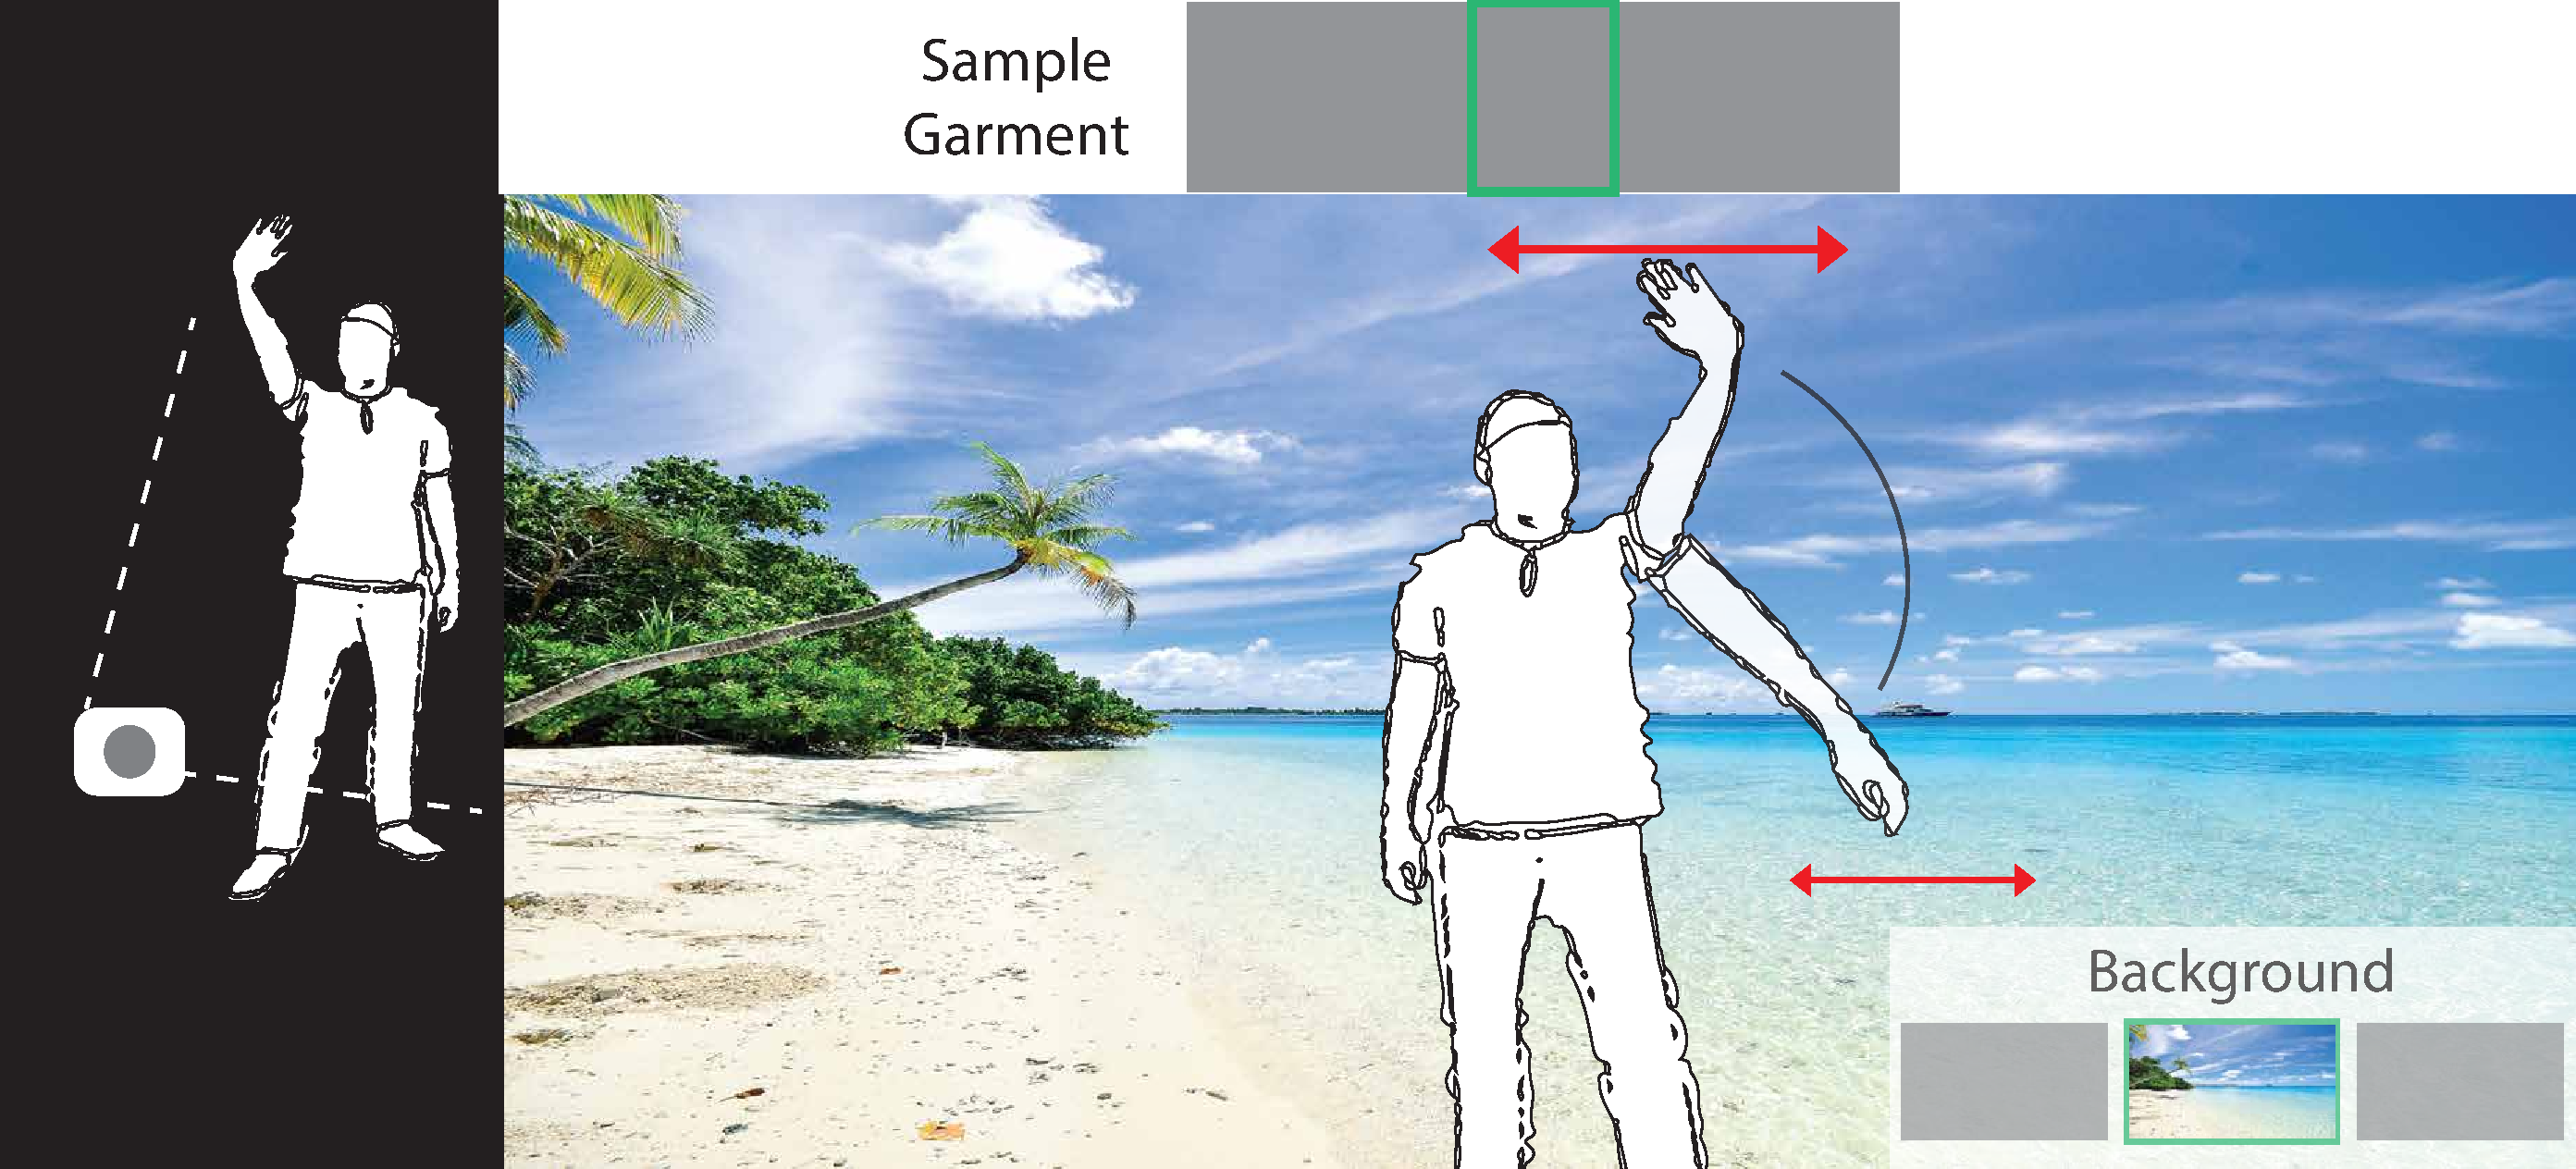
\includegraphics[width=\textwidth]{content/resources/images/application/ar-instruction.pdf}
  \caption{Instruction of Magic Mirror}
  \label{fig:ar-instruction}
\end{figure}

The user interface (UI) of Magic Mirror consists of the following parts (as shown in~\autoref{fig:ar-instruction}): the interaction area, the garment and the background display area. We prepare a list of in-shop garments and backgrounds that users can choose according to their needs.

The interaction area is the main display part of our application. First, the camera captures and displays the user's image in this area. And depending on the chosen outfit, the virtual try-on result is displayed correspondingly. If they want to change clothes, the users can use hand gestures to slide on the upper half of the interaction area to choose their desired item. And similarly, they can also use the slider gestures to change the background but on the lower half of the screen (as illustrated in~\autoref{fig:ar-instruction}). Some examples of the capabilities of this application are demonstrated in~\autoref{fig:ar-ui}

\begin{figure}[ht]
    \centering
    \subfloat[]{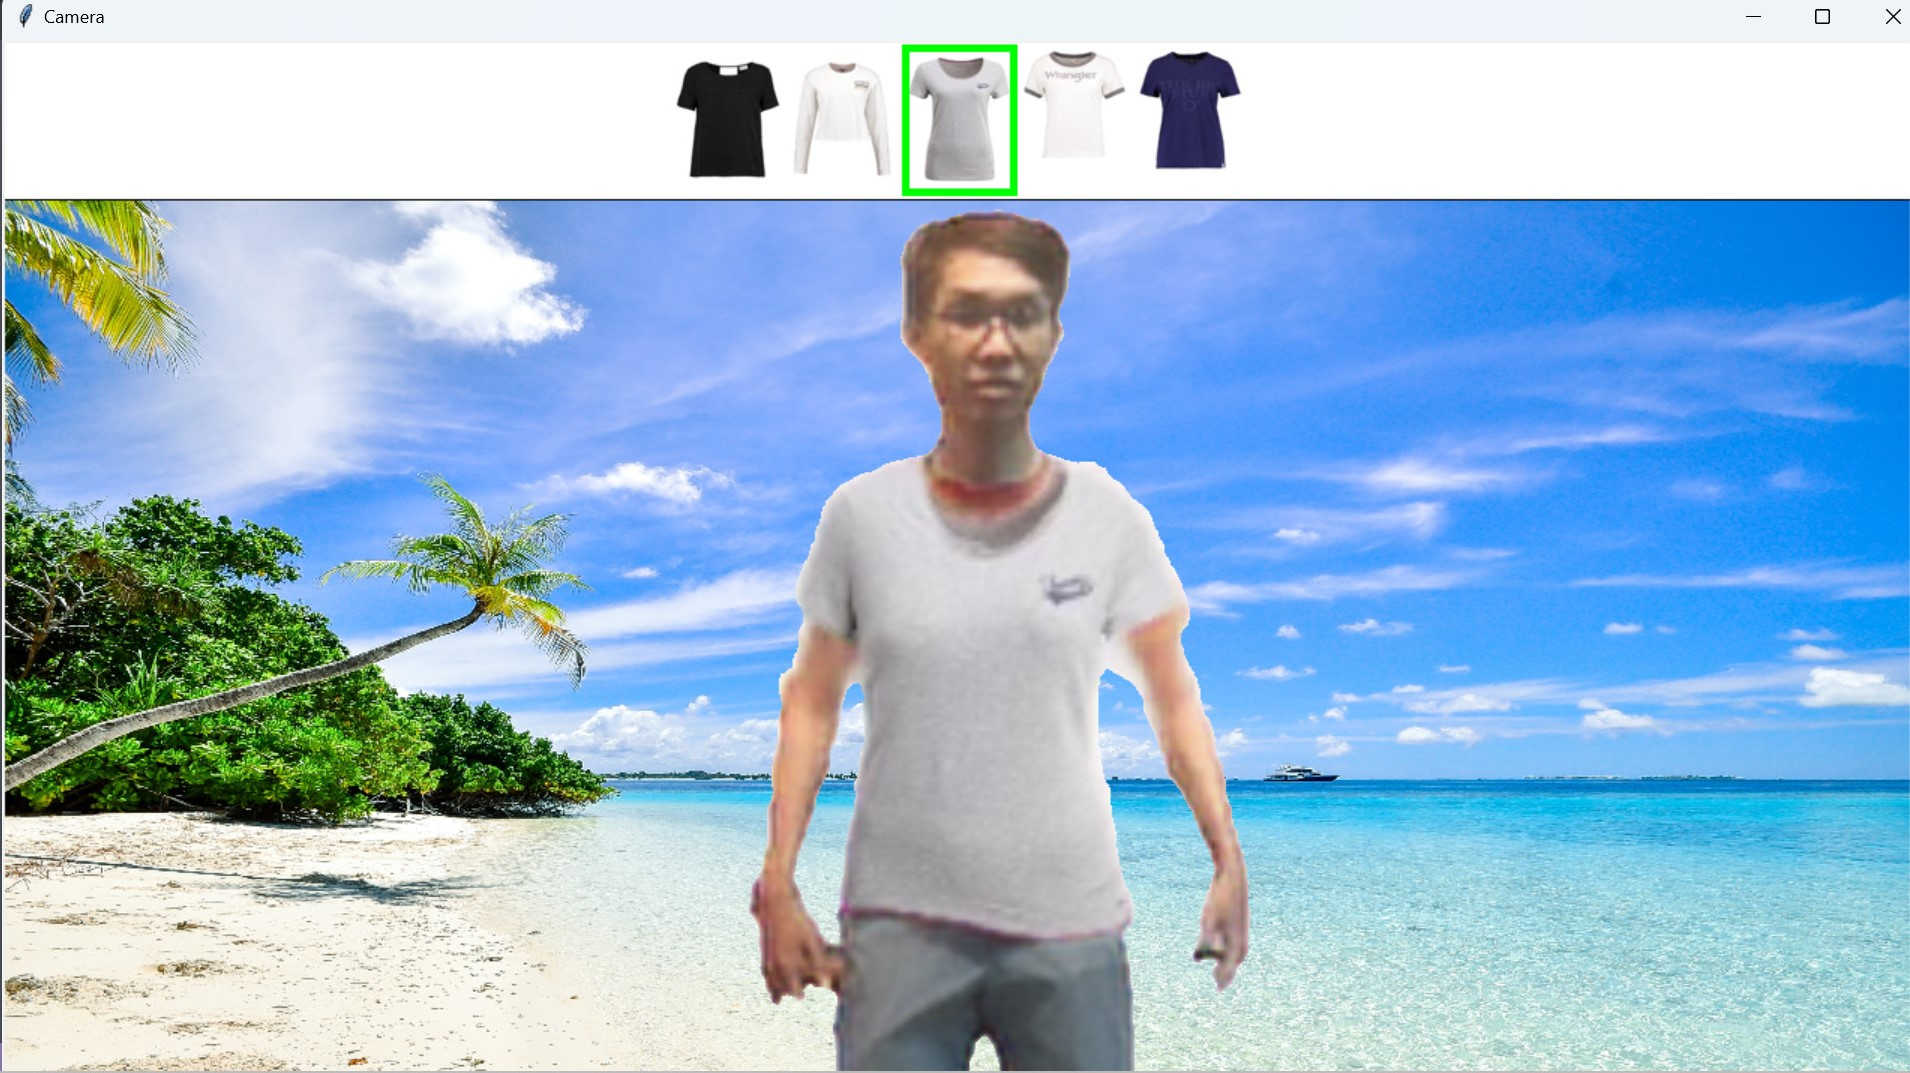
\includegraphics[width=0.5\columnwidth]{content/resources/images/application/ar-ex1.jpg}}
    \subfloat[]{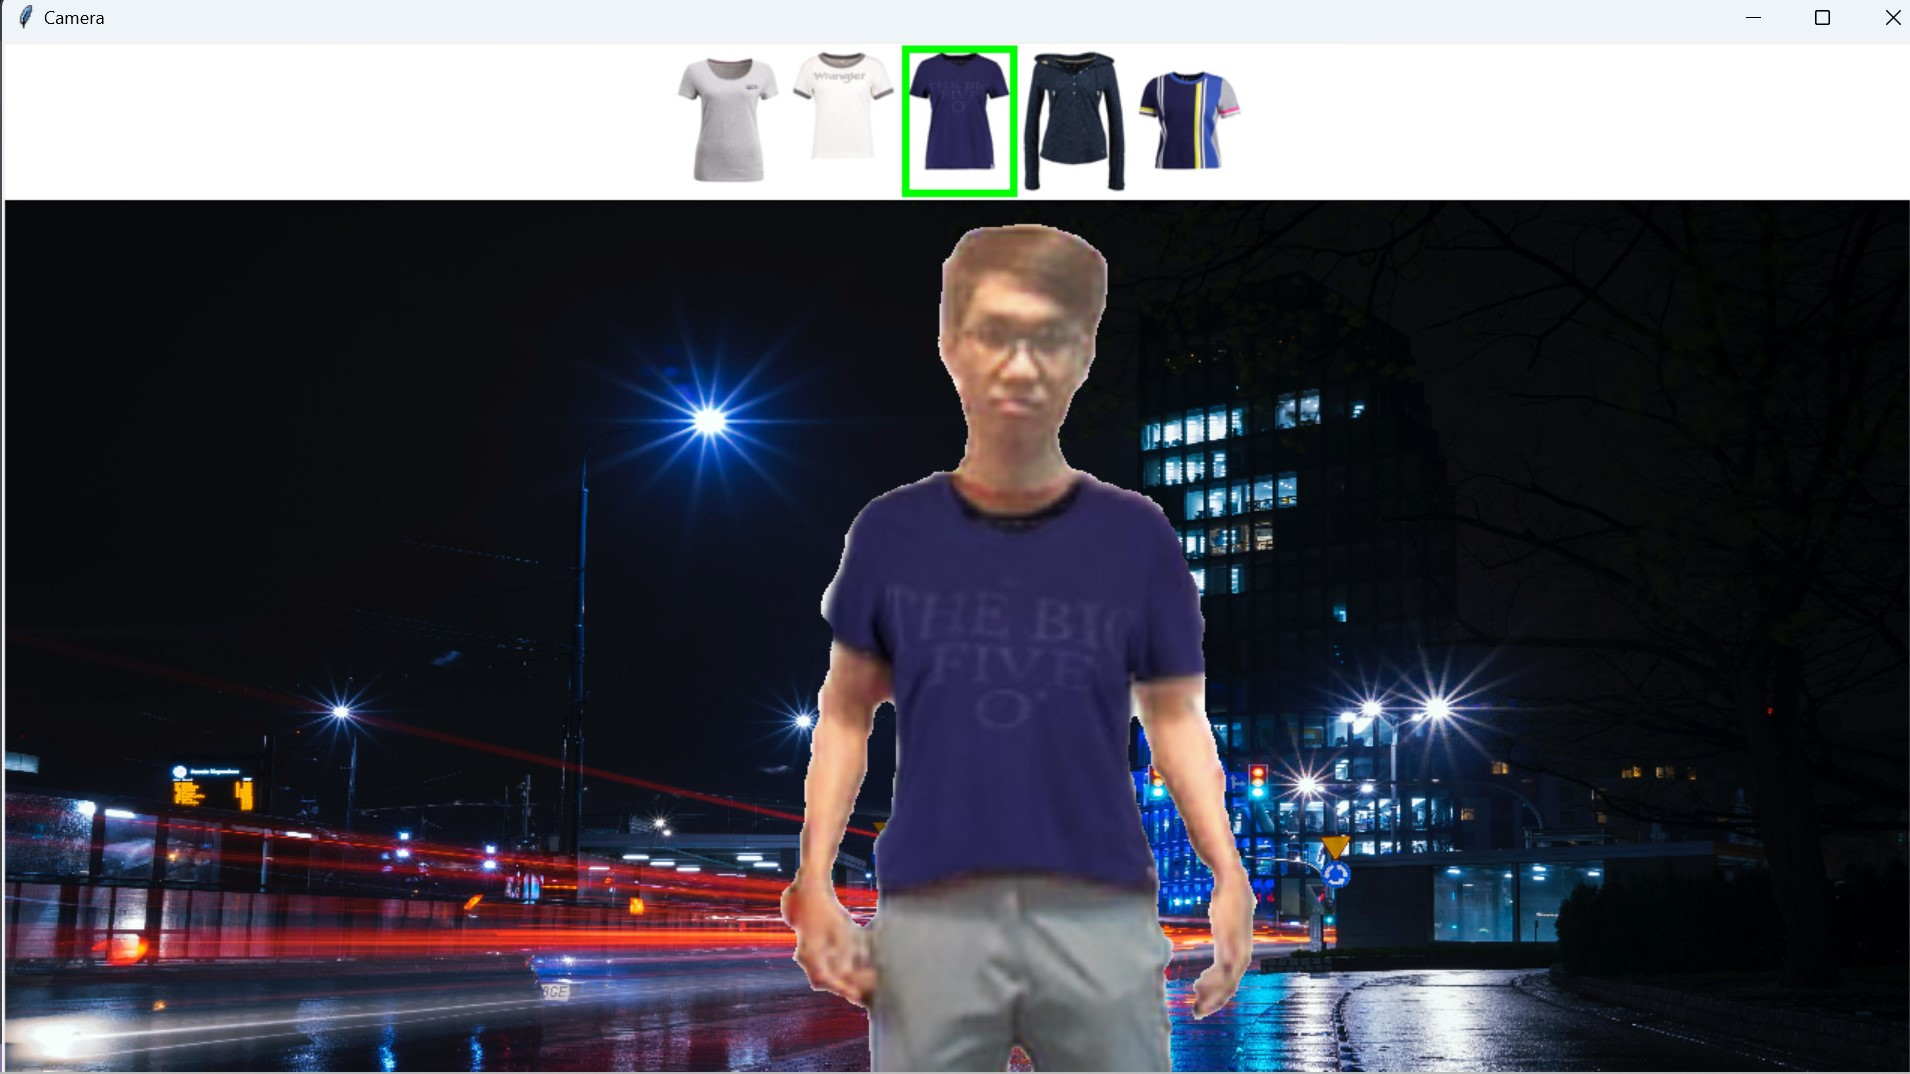
\includegraphics[width=0.5\columnwidth]{content/resources/images/application/ar-ex2.jpg}} 
    \caption{The UI of Magic Mirror}
    \label{fig:ar-ui}
    \vspace{-2mm}
\end{figure}

\section{Smart Fashion Assistant System}

\subsection{Overview}
 We demonstrate the scenario where users find a particular garment that catches their eye while shopping online at home. They consider buying it but are unsure whether it looks good on them. We facilitate it by offering the Smart Fashion Assistance system. Using this system, users can try on such garments before purchasing. Upon try-on, the system recommends other fashion items that may suit their tastes and preferences. Users can also find new garments with some relative attributes (i.e. green, longer sleeves) to the selected garment by providing feedback in natural language. \autoref{fig:web-flow} illustrates how our system works.

 \begin{figure}[h!]
  \centering
  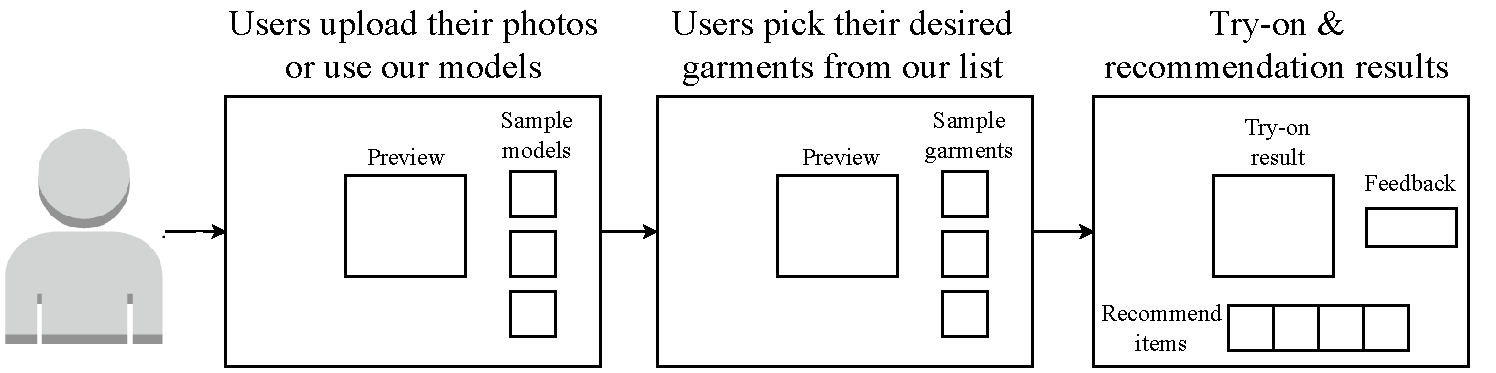
\includegraphics[width=\textwidth]{content/resources/images/application/chapter5-web-flow.pdf}
  \caption{Demo overview of Smart Fashion Assistant System}
  \label{fig:web-flow}
\end{figure}

\begin{figure}[b!]
    \centering
    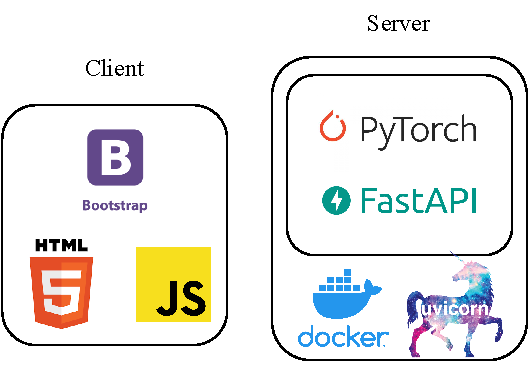
\includegraphics{content/resources/images/application/chapter5-web-arch.pdf}
    \caption{The architecture of Smart Fashion Assistance system}
    \label{fig:chapter5-web-arch}
\end{figure}

\subsection{Implementation details}
Specifically, we develop the Smart Fashion Assistant system utilizing a client-server architecture~\autoref{fig:chapter5-web-arch}. We build the client user interface with HTML, Bootstrap, and Javascript to bring out the best user experiences on the browser. We develop our deep learning models in the back-end server utilizing the PyTorch framework~\cite{Paszke-NeurIPS2019-Pytorch}. We also incorporate the HNSW search algorithm using the FAISS implementation. The HTTPS entry points are handled by the FastAPI framework. We utilize Uvicorn, a Python implementation of an ASGI web server, to serve the server. Finally, we package the entire server using Docker and deploy it on a cloud service with an NVIDIA A100 GPU.

\subsection{Usage and Examples}
\begin{figure}[h]
  \centering
  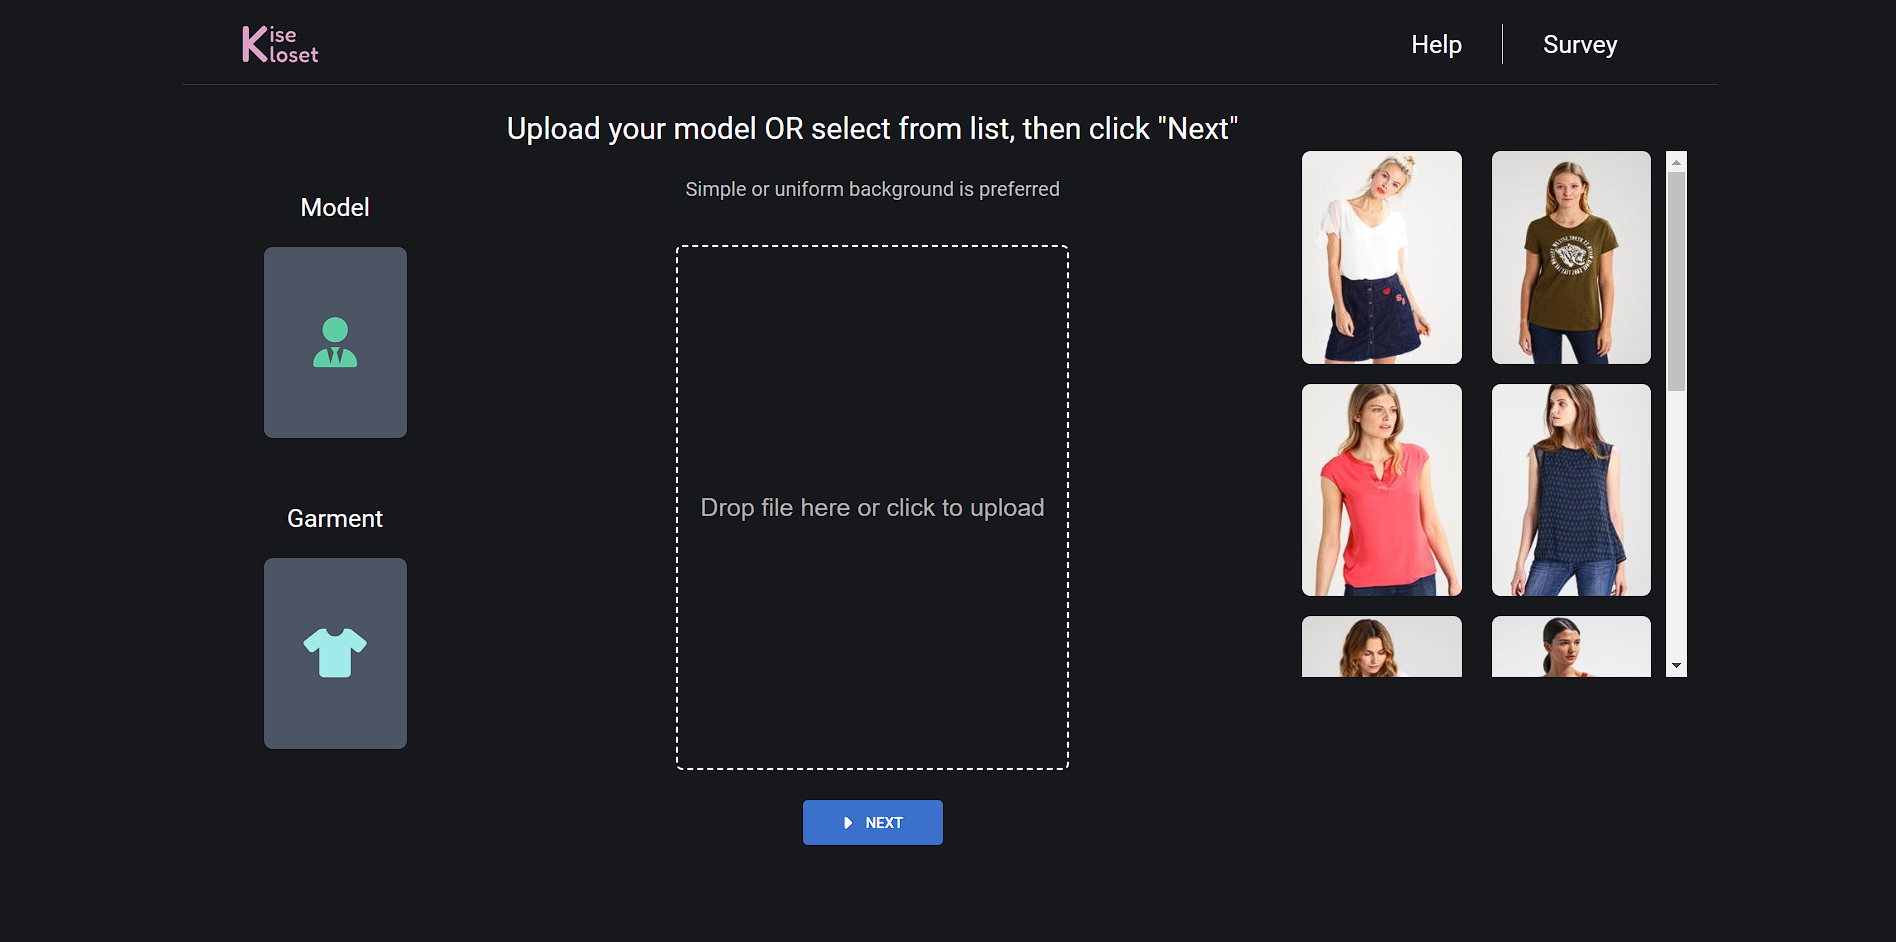
\includegraphics[width=\textwidth]{content/resources/images/application/web-step0.png}
  \caption{The initial UI of Smart Fashion Assistance system}
  \label{fig:web-step0}
\end{figure}

Upon entering the website, users are presented with the user interface (UI) displayed in Figure \ref{fig:web-step0}. We prepare some human models beforehand as references for users. They can use those models or upload their photos as input images for the try-on framework. \autoref{fig:web-step1} demonstrates the case where a user picks one of our provided models. After that, users can press the Next button below to advance to the next step.

Subsequently, users must upload or pick the garment they want to try on from our provided list on the right side (as shown in~\autoref{fig:web-step2}). The left panel also displays the chosen model image in the previous step. Now users can press the Next button to view the try-on result. 

\begin{figure}[h]
  \centering
  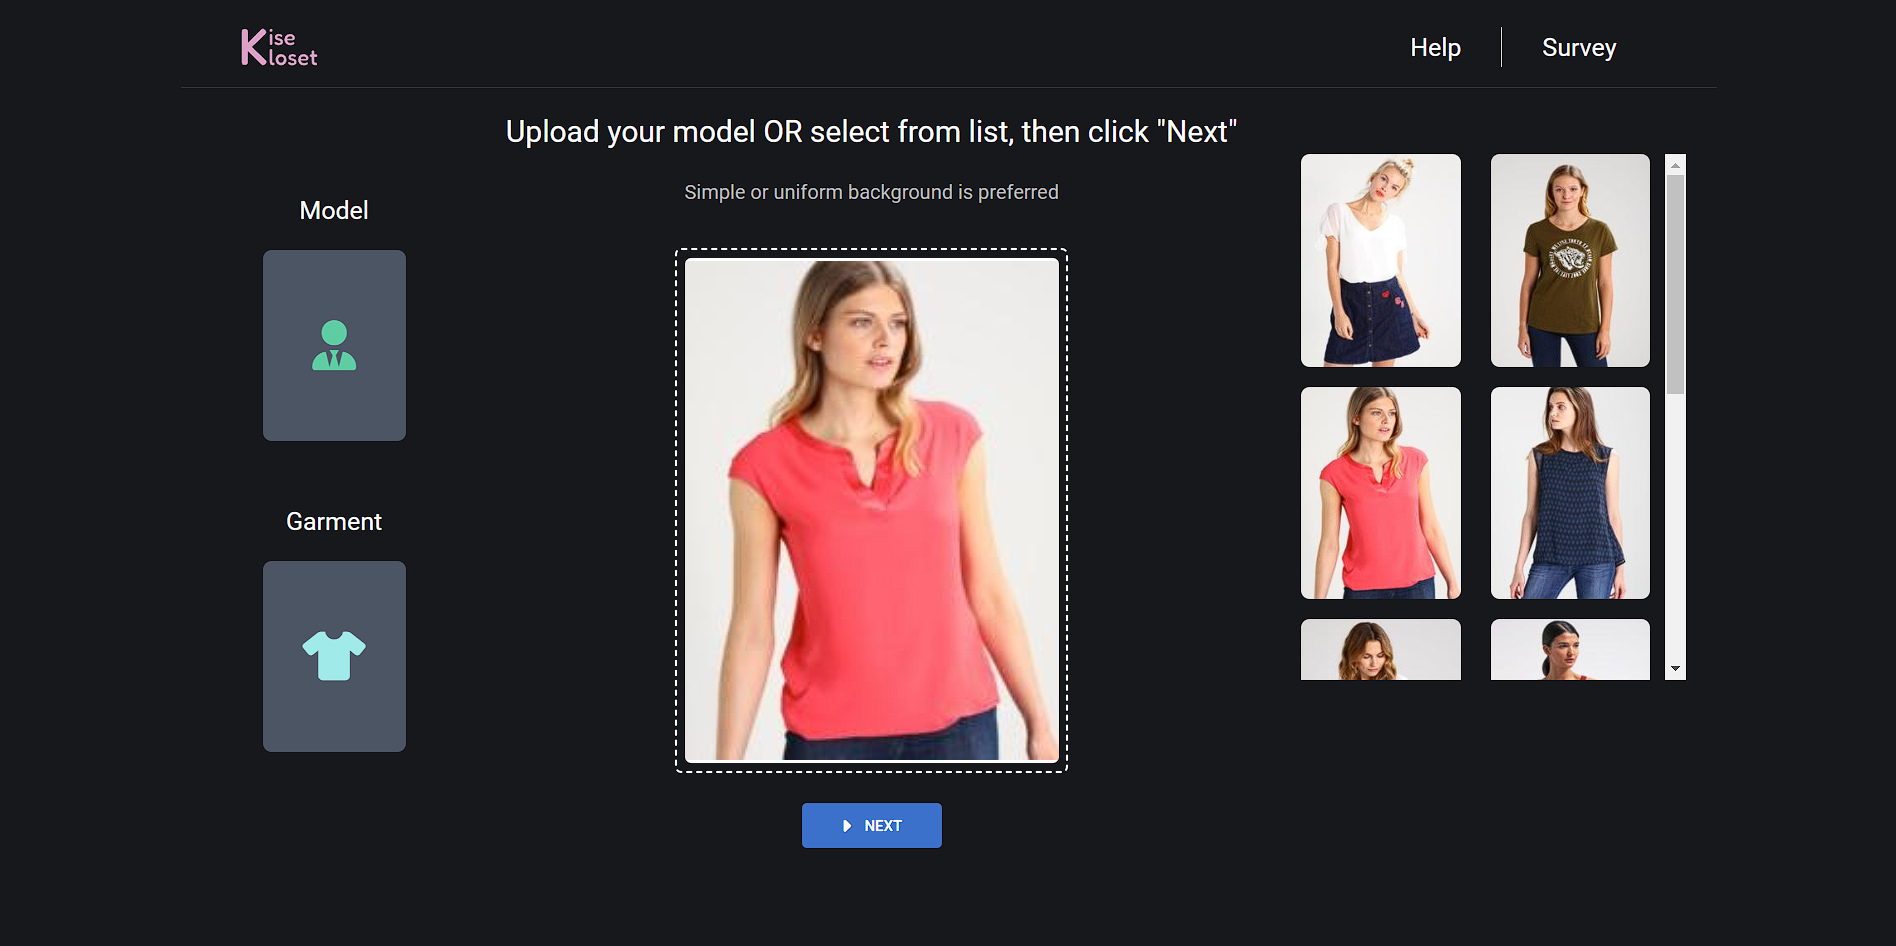
\includegraphics[width=\textwidth]{content/resources/images/application/web-step1.png}
  \caption{Choose the input person to try on. An example where a user picks one of our provided models}
  \label{fig:web-step1}
\end{figure}

\begin{figure}[h!]
  \centering
  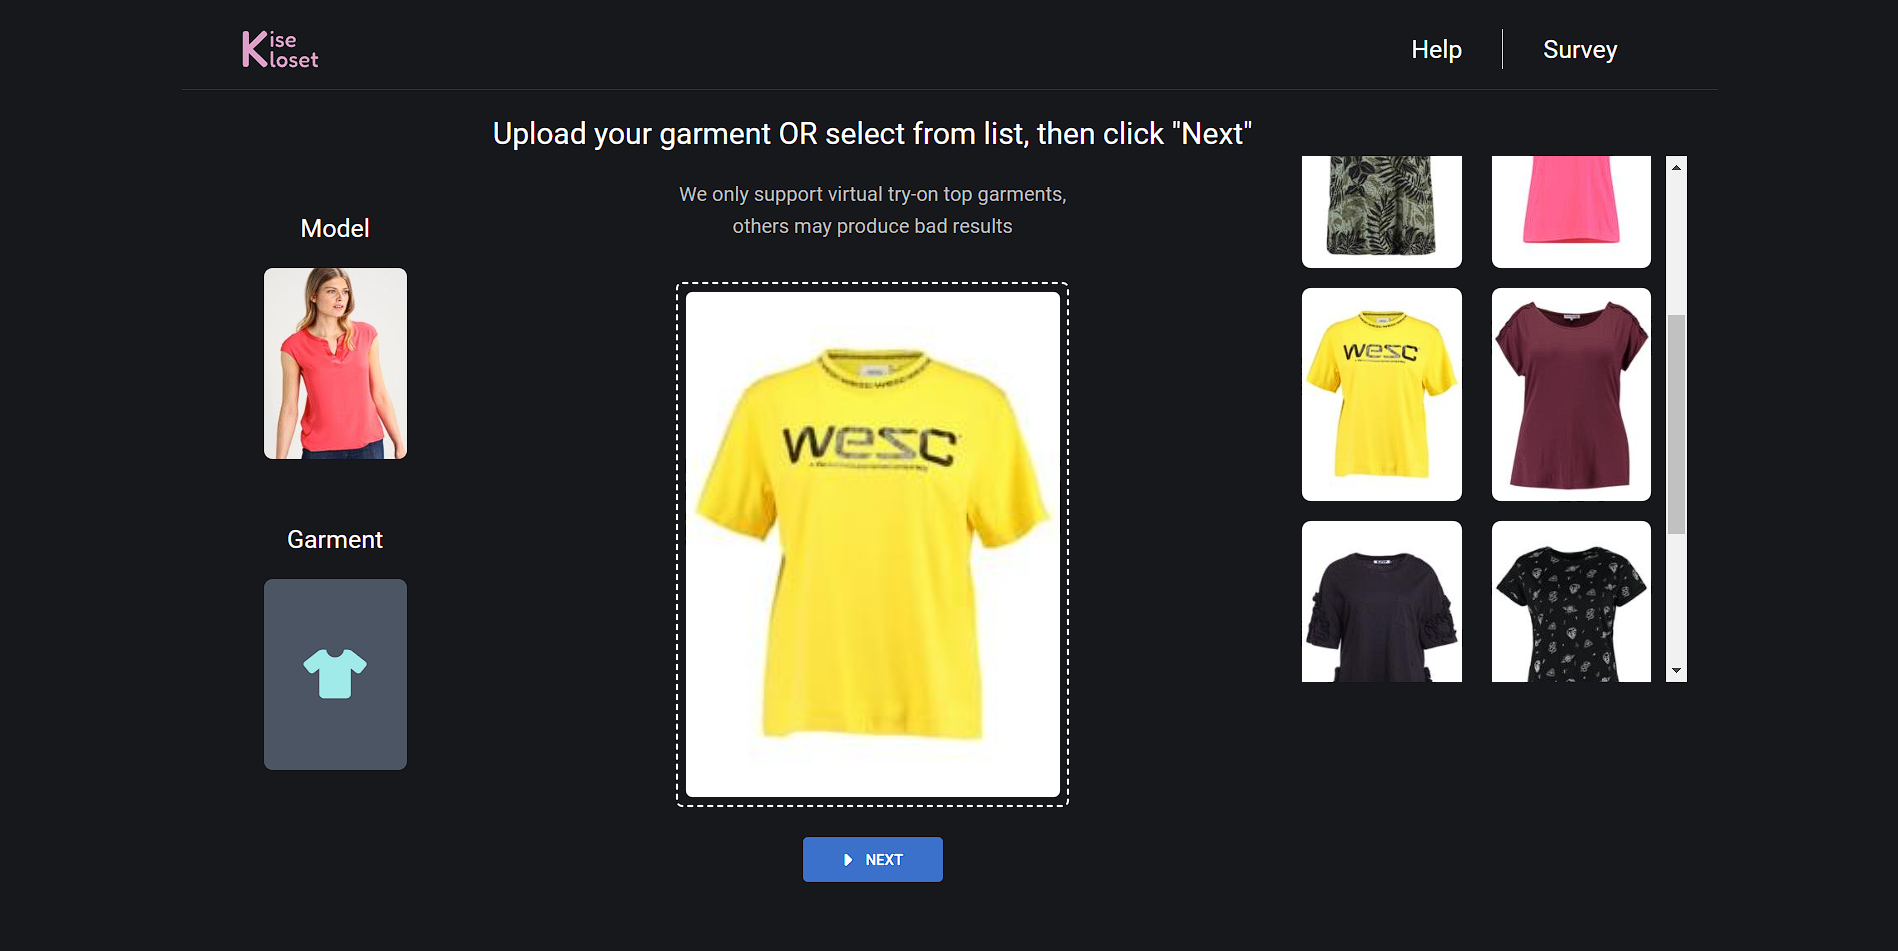
\includegraphics[width=\textwidth]{content/resources/images/application/web-step2.png}
  \caption{Choose the target garment to try on. Users must pick one of the garments provided on the right panel}
  \label{fig:web-step2}
\end{figure}

Once users have chosen both the input person and garment image, they are presented with the try-on result, as shown in \autoref{fig:web-recommend}. A slider in the middle allows users to compare the original and try-on images. Beneath the try-on result, we provide recommendations for the chosen garment. These recommendations include items within the same category as the reference item and items from other categories that may catch users' attention. Users can try on these recommended items by clicking on them, but we currently only permit selecting items within the same category. As for items from other categories, we provided 2 options: Ton sur ton, items with the same color or textures, and, hipster style, items with mixed style and color. In case users want garments not included in the recommendation list but have some relation to the reference item, we offer a text box on the right side. Users can input their preferences; consequently, we provide new item recommendations based on their feedback.

\begin{figure}[h!]
  \centering
  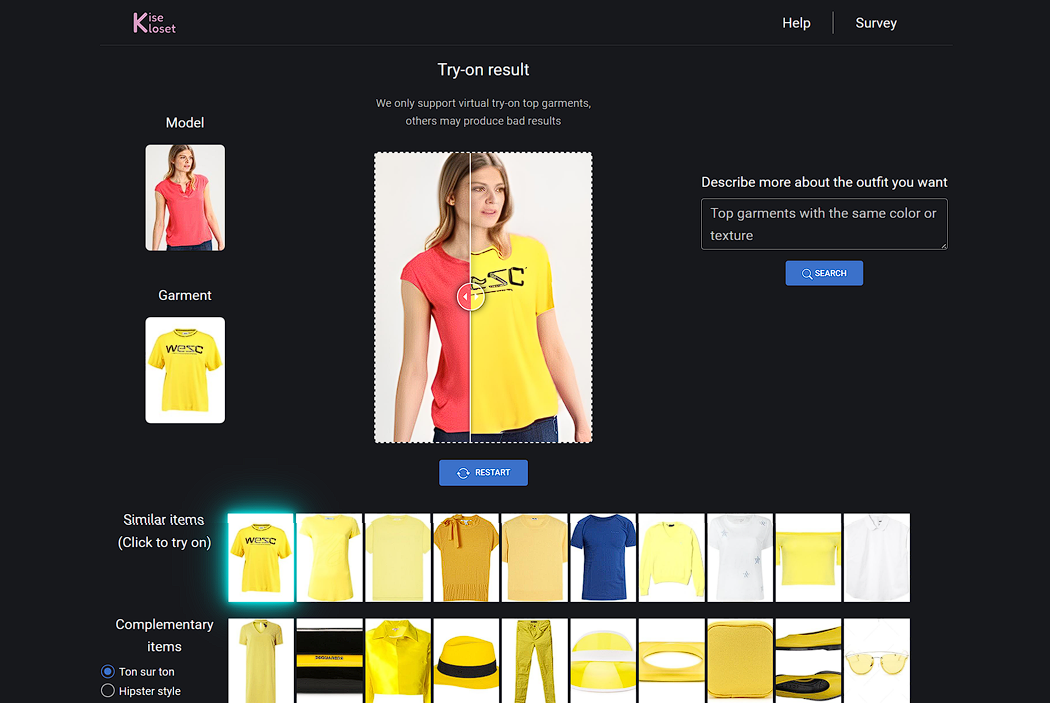
\includegraphics[width=\textwidth]{content/resources/images/application/web-recommend.png}
  \caption{Try-on result and recommendation playground}
  \label{fig:web-recommend}
\end{figure}

\section{Experiments}
\subsection{Workflow Overview}
\begin{figure}[h!]
  \centering
  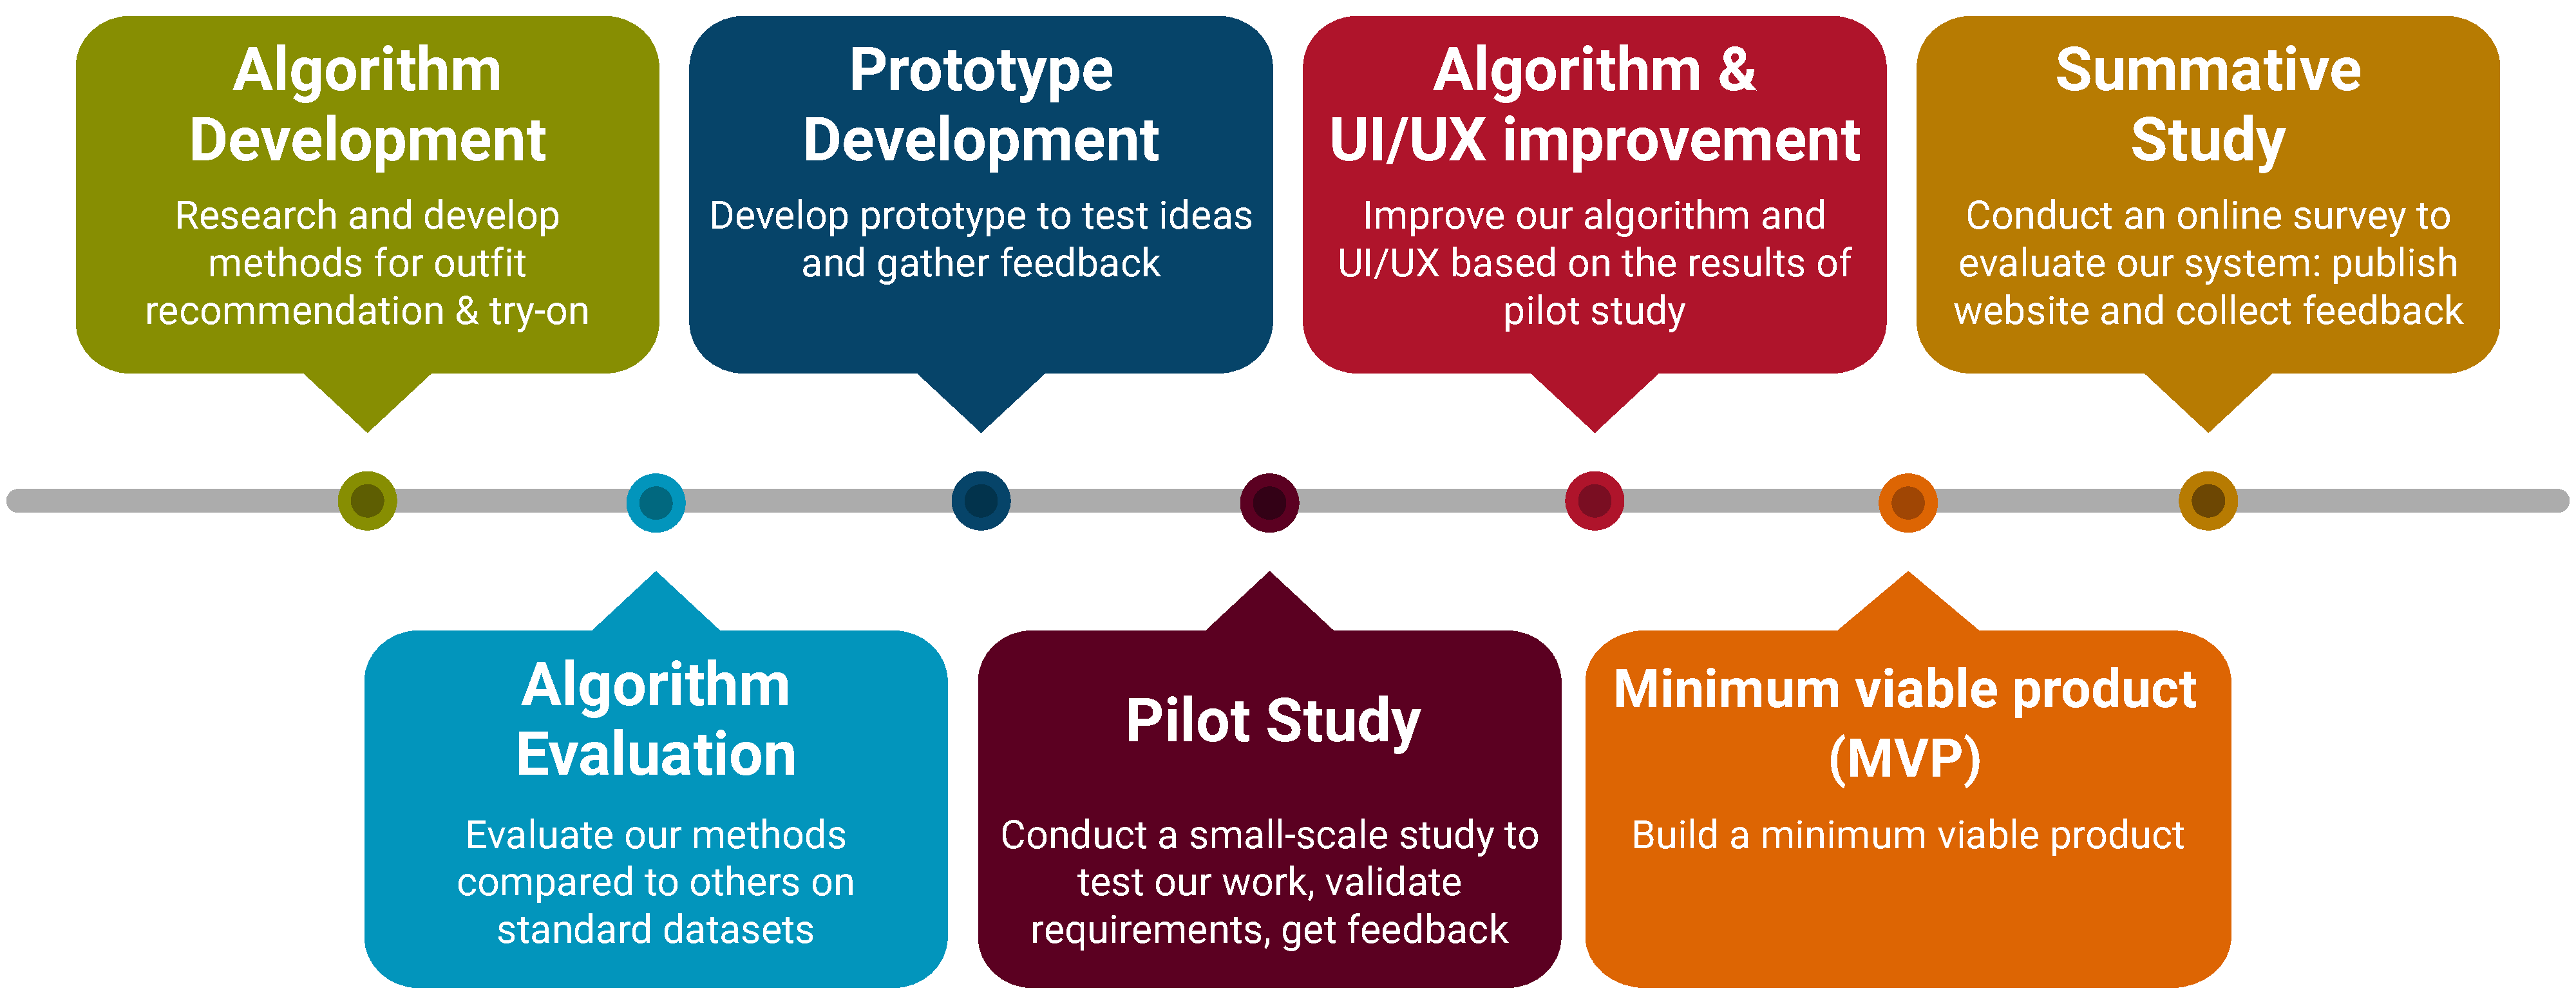
\includegraphics[width=\textwidth]{content/resources/images/application/workflow.pdf}
  \caption{Workflow of development.}
  \label{fig:exp-workflow}
\end{figure}
We follow the workflow shown in~\autoref{fig:exp-workflow} during application research and development. The research workflow described here presents a comprehensive and iterative process to develop and refine algorithm and user experience (UX) design, leading to the creation of a viable product. The workflow comprises seven key stages: algorithm development, algorithm evaluation, prototype development, pilot study, algorithm \& UI/UX improvement, minimum viable product (MVP), and summative study.

In the first stage, algorithm development, we focus on researching and developing algorithms for the virtual try-on and outfit recommendation problems. This stage involves reviewing existing literature, identifying knowledge gaps, and iterative experimentation to devise our approach. Following this, rigorous assessments of the developed algorithms' efficacy and performance are undertaken in the algorithm evaluation stage. We conduct various tests and benchmarking procedures on standard datasets to evaluate the effectiveness of our proposed methods. The works done during the first two stages create a solid foundation for subsequent steps. The outcomes of these stages are documented and presented in~\autoref{chapter-literature-review},~\autoref{chapter-virtual-tryon}, and~\autoref{chapter-fashion-recommendation}.

Subsequently, the research progresses to the stage of prototype development. A rudimentary prototype is constructed, wherein the algorithm is integrated into a user interface. This version enables the execution of a pilot study with a small group of participants to gather valuable feedback about the algorithm's efficacy and the user interface/user experience (UI/UX) design. The detailed report of this pilot study can be found in~\autoref{app-exp-pilot-study}. The outcomes of this preliminary study help us identify existing issues and areas for enhancing the efficacy of our research.

After a small-scale study, we utilize the acquired insights to improve our system. Successive enhancements were implemented to optimize the algorithm's accuracy and performance, while concurrently refining the UI/UX to improve user satisfaction. Subsequently, integrating these improvements, a minimum viable product (MVP) was developed, representing a more advanced version of the initial prototype (see~\autoref{fig:web-ui-before-after}).

\begin{figure}[h!]
  \centering
  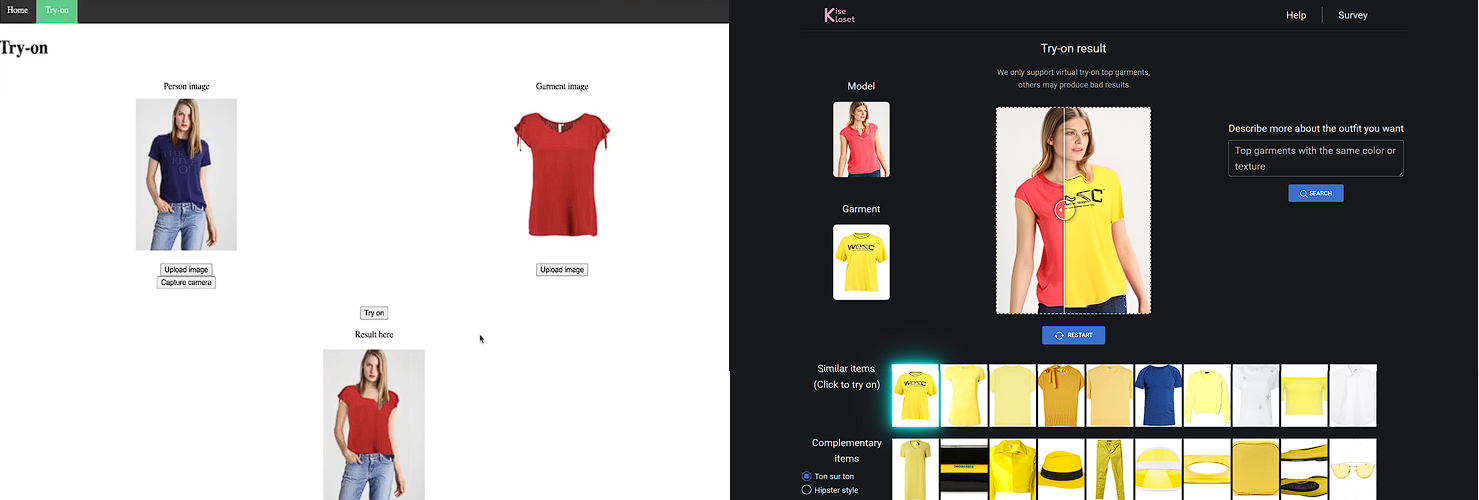
\includegraphics[width=\linewidth]{content/resources/images/application/web-before-after.png}
  \caption{Smart Fashion Assistant UI comparison before and after improvements (left: prototype, right: MVP)}
  \label{fig:web-ui-before-after}
\end{figure}

Finally, we conduct a large-scale summative study to assess our MVP from the end-user's perspective. We open web access and invite online users to participate in trials and surveys. The valuable insights and opinions collected from these users play an important role in objectively evaluating the system. This study provides evidence of the system's effectiveness, validates its algorithmic capabilities, and measures user satisfaction, ensuring our application is viable. Further specifics about this study can be found in~\autoref{app-exp-summative-study}.

In summary, this research workflow offers a systematic approach to developing and perfecting algorithms and UI/UX design, ensuring an efficient and user-friendly website is created. The iterative nature of the process allows for continuous refinement and optimization, leading to a well-validated product.

\subsection{Pilot Study}
\label{app-exp-pilot-study}
We invited 12 participants who are university students and researchers in the 18-44 age range. We let the users experience our Smart Fashion Assistance system and collected their feedback.

Regarding the available garments, we prepared a collection of 20 garments taken from the VITON~\cite{Han-CVPR2018-Viton} and PolyvoreOutfits~\cite{Mariya-ECCV18-Learning} datasets (see~\autoref{fig:pilot-study-data}). These garments were carefully selected to represent a variety of colours, shapes, and textures.

Each participant took part in a 10-minute session in which the participant was asked to perform a virtual try-on using our provided model images and virtual try-on on themselves directly captured from our camera. In terms of human models, we used 10 person images in the VITON~\cite{Han-CVPR2018-Viton} and DeepFashion~\cite{Liu-CVPR2016-DeepFashion} datasets (see~\autoref{fig:pilot-study-data}).

\begin{figure}[h!]
    \centering
    \subfloat[Human model samples]{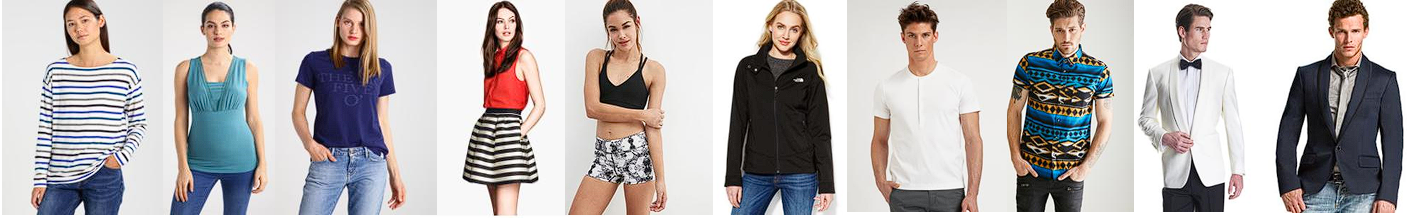
\includegraphics[width=\columnwidth]{content/resources/images/application/study-model.png}} \\
    \subfloat[Garment samples]{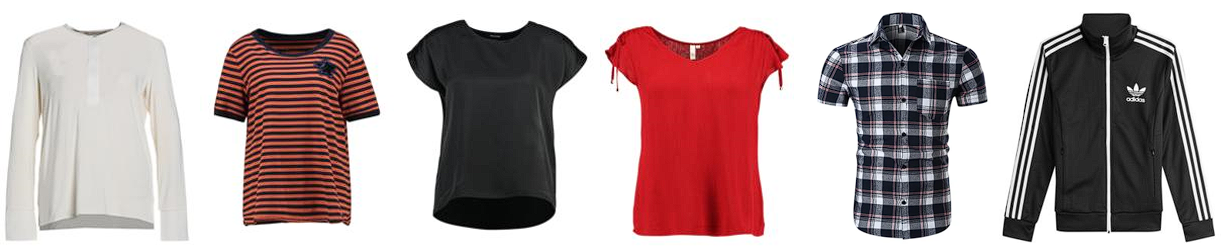
\includegraphics[width=\columnwidth]{content/resources/images/application/study-sample.png}}
    \caption{Examples of data used in our pilot study.}
    \label{fig:pilot-study-data}
    \vspace{-2mm}
\end{figure}

Upon completing the trial, we interviewed participants and asked for their feedback. Our primary objective was to evaluate how our system influenced their purchasing decisions. We also gathered their feedback about the output quality and whether they prefer using the model images or their own images to enhance the overall user experience in the future.

\begin{figure}[h!]
  \centering
  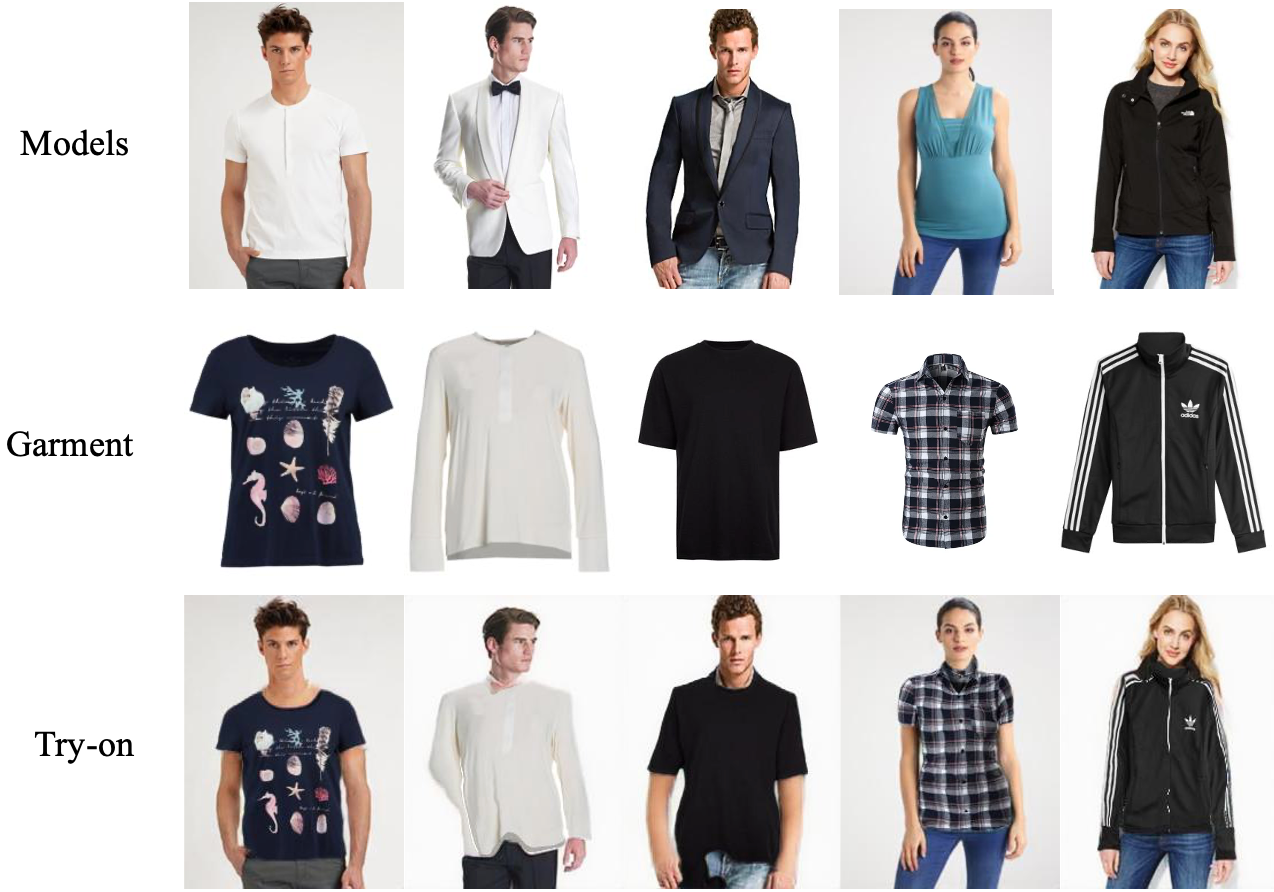
\includegraphics[width=0.8\linewidth]{content/resources/images/application/study-result.png}
  \caption{Results obtained when users performed virtual try-on on our provided human models in the pilot study.}
  \label{fig:study-result}
  \vspace{-2mm}
\end{figure}

Most of the participants agreed that trying on clothes in various poses helped them visualize the suitability of the garments before making a purchase decision. Specifically, $66.7\%$ of the participants felt confident enough to make the purchasing decision after using our system, while the remaining $33.3\%$ had doubts about the truthiness of the models. Moreover, $83.3\%$ of the participants preferred using their images for try-on, as it provided a more realistic experience for them. On the other hand, the remaining $16.7\%$ considered both options, as the provided models allowed them to see the best representation of the garments, such as with appropriate brightness and poses.~\autoref{fig:study-result} illustrates some virtual try-on results on our provided models. Due to privacy issues, we did not capture the virtual try-on results on the participants' images.

We also received valuable feedback from participants on areas for improvement. In real-life conditions, the background, brightness, and quality of the captured images might not be suitable for trying on clothes, which is due to the fact that our train and test datasets only contain simple backgrounds and have proper brightness conditions. Thus, applying some pre-processing techniques such as segmentation and brightness equalization is necessary to address this issue. Additionally, participants also suggested that our system exhibited inconsistencies when dealing with complex poses such as half-turn poses or crossed-arm poses. Their feedback is useful in enhancing the user experience in the future.

% _ Pilot study: vẽ thêm workflow: prototype -> pilot study -> final product (hay dùng chữ gì tùy) -> user study
% Mục đích: pilot study để lấy phản hồi nhằm improve thiết kế (interface & interaction) để tăng cường trải nghiệm người dùng


\subsection{Summative Study}
\label{app-exp-summative-study}
\begin{figure}[h!]
  \centering
  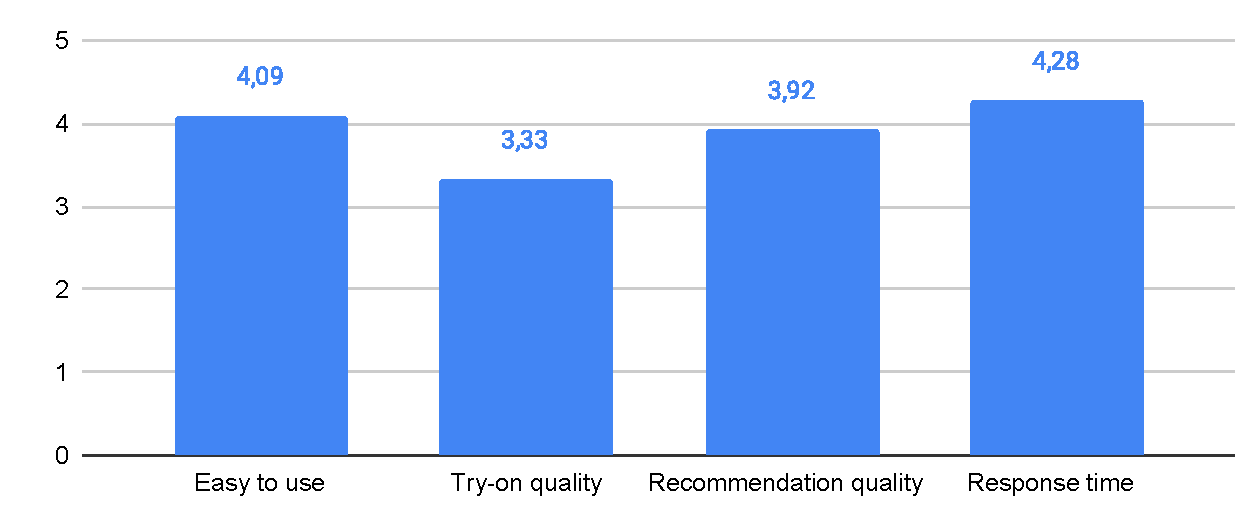
\includegraphics[width=0.8\linewidth]{content/resources/images/application/exp-user-overall.pdf}
  \caption{Average rating scores from the user study evaluation (1: very dissatisfied, 5: very satisfied)}
  \label{fig:user-overall}
\end{figure}

We deployed our system at \url{http://selab.edu.vn:20440/} for online users to try out and provide feedback. Our survey primarily aimed to measure users' satisfaction in four key factors: ease of use, try-on quality, recommendation quality, response time, and response time. \autoref{fig:user-overall} shows the average rating scores of each factor on a scale of 1 to 5 (1: very dissatisfied, 5: very satisfied) from the user study evaluation, which indicates that those users had a positive overall experience with our website.

\begin{figure}[h!]
  \centering
  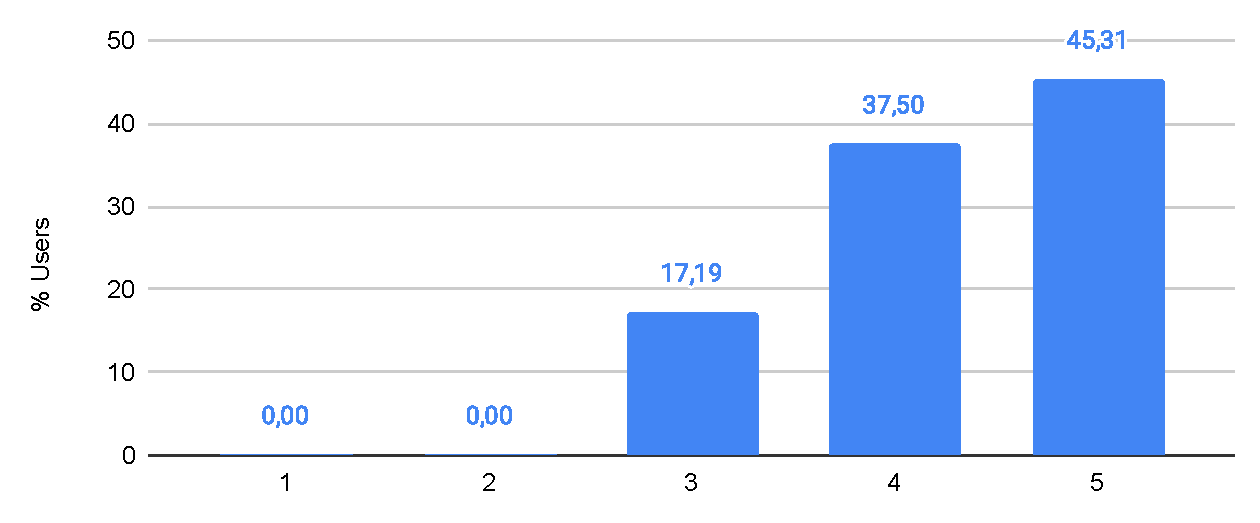
\includegraphics[width=0.8\linewidth]{content/resources/images/application/exp-user-response-time.pdf}
  \caption{Rating scores of response time (1: very dissatisfied, 5: very satisfied)}
  \label{fig:response-time}
\end{figure}

Regarding the response times, it received the highest rating among the four factors, followed by ease of use.  As shown in \autoref{fig:response-time}, almost all users expressed their satisfaction with the response time. This aspect was our primary focus during the development of the deep learning models, as we prioritized optimizing the inference speed to deliver quicker results.

Regarding the quality of the results, most users either expressed satisfaction or had a neutral attitude towards the try-on output, as indicated in~\autoref{fig:tryon-quality} and~\autoref{fig:tryon-howvisualize}. Positive feedback highlighted the superb try-on quality, as it effectively assisted users in visualizing the garments in action, providing them with a valuable tool for making fashion choices.

\begin{figure}[h!]
  \centering
  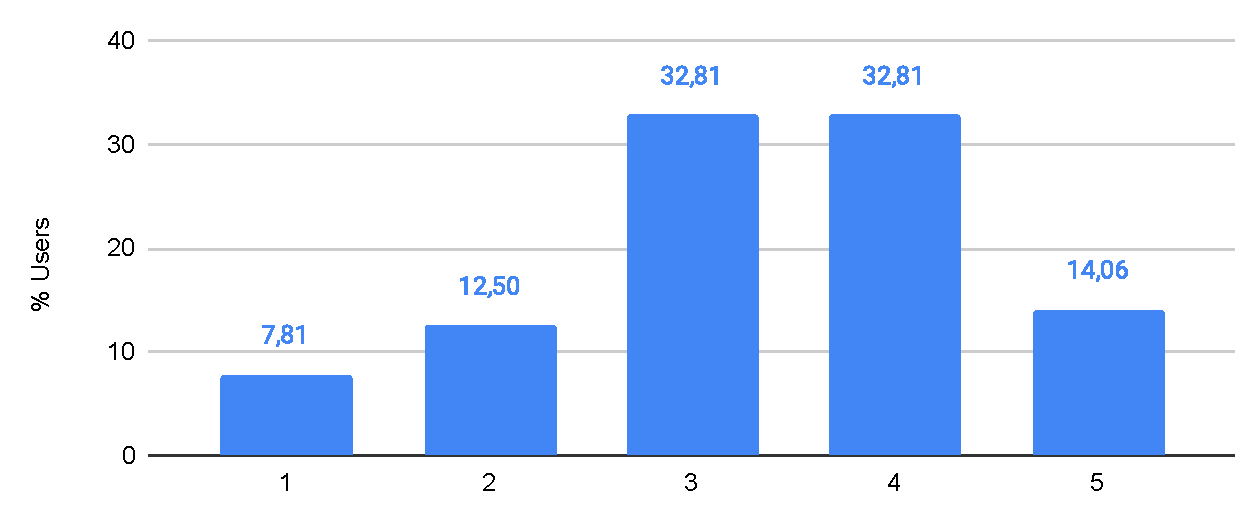
\includegraphics[width=0.8\linewidth]{content/resources/images/application/exp-user-tryon-quality.pdf}
  \caption{Rating scores of try-on quality (1: very dissatisfied, 5: very satisfied)}
  \label{fig:tryon-quality}
\end{figure}

\begin{figure}[h!]
  \centering
  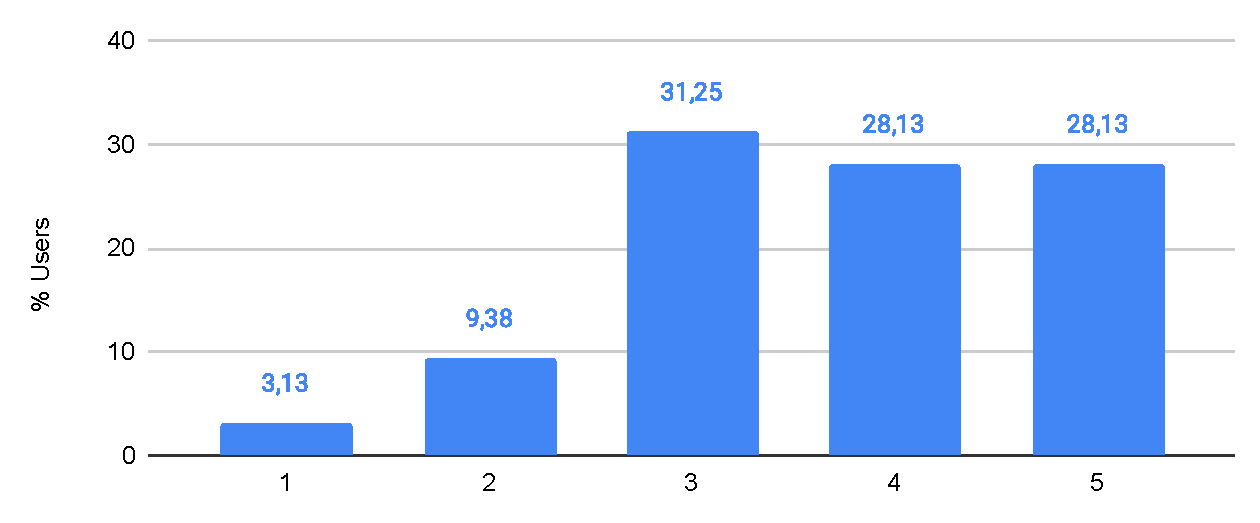
\includegraphics[width=0.8\linewidth]{content/resources/images/application/exp-user-tryon-howvisualize.pdf}
  \caption{Statistics of user answers to questions: Do you agree that the virtual try-on feature helps you visualize the garment's appearance when you wear it? (1: completely disagree, 5: completely agree)}
  \label{fig:tryon-howvisualize}
\end{figure}

As for the recommendation results, the rating scores in \autoref{fig:rec-result} indicated users' satisfaction with them, highlighting the positive impact of the feedback-based item recommendation on enhancing the overall user experience. This feature helped users receive recommendations that align with their unique tastes and preferences, making their shopping journey more enjoyable and efficient.

\begin{figure}[h!]
  \centering
  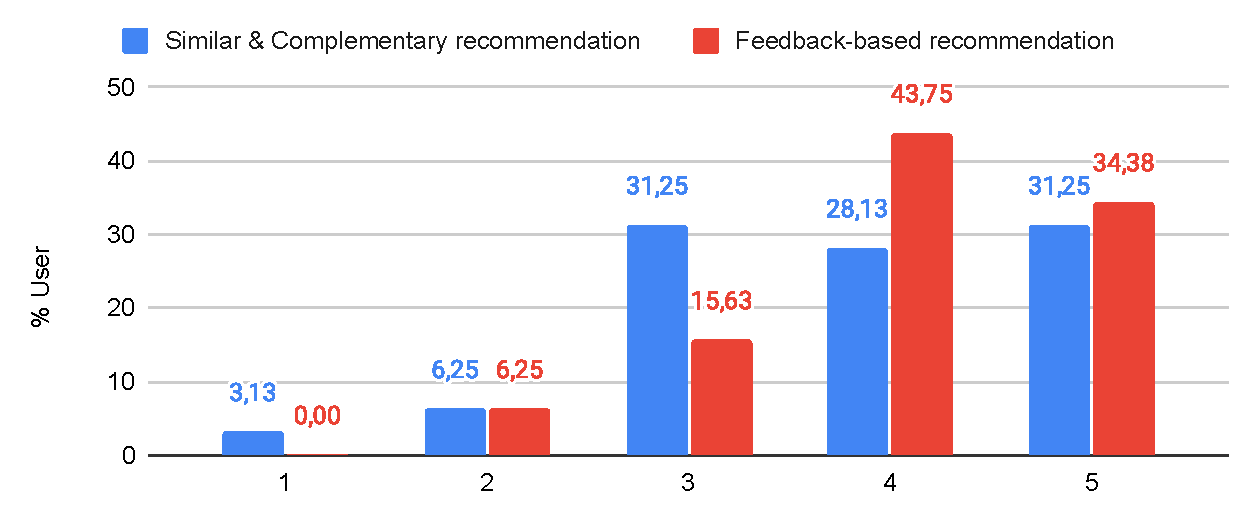
\includegraphics[width=0.8\linewidth]{content/resources/images/application/exp-user-rec-result.pdf}
  \caption{Rating scores on recommendation quality (1: very dissatisfied, 5: very satisfied)}
  \label{fig:rec-result}
\end{figure}

Moreover, the user study revealed that 84,375\% of users found our system highly useful and effectively improved their online shopping experience. Furthermore, 65,625\% of the users expressed their willingness to recommend our system to their friends and family, emphasizing the positive reception and satisfaction among users. 

Especially, we also get positive comments from experts in the industry, such as Mr. Le Tan Dang Khoa, a research software engineer at ViSenze, a leading company in Singapore known for providing AI solutions for visual commerce such as visual recommendation, augmented reality, and virtual try-on. He commends the system for its intuitive user interface, effectively catering to the diverse requirements of online shoppers. He further evaluates that with a few adjustments and fine-tunings, the system has the potential to transform into a minimum viable product suitable for integration within any e-commerce shop.

In conclusion, our system offers a comprehensive end-to-end solution for virtual try-on, accompanied by valuable additional features such as fashion recommendation, and text feedback-based search. The seamless and fast visual search ensures that similar and complementary items are promptly displayed without delays. As we continue to collect and analyze user feedback, we remain committed to improving our system further to ensure that our platform continues to deliver exceptional virtual try-on experiences and personalized fashion recommendations for our valued users.


\section{Limitations \& Discussions}
Despite receiving positive feedback, it is essential to acknowledge the limitations of the Smart Fashion Assistance application. Through an analysis of negative feedback obtained from the summative study and previous evaluation experiments, several shortcomings have been identified.

\begin{figure}[h!]
    \centering
    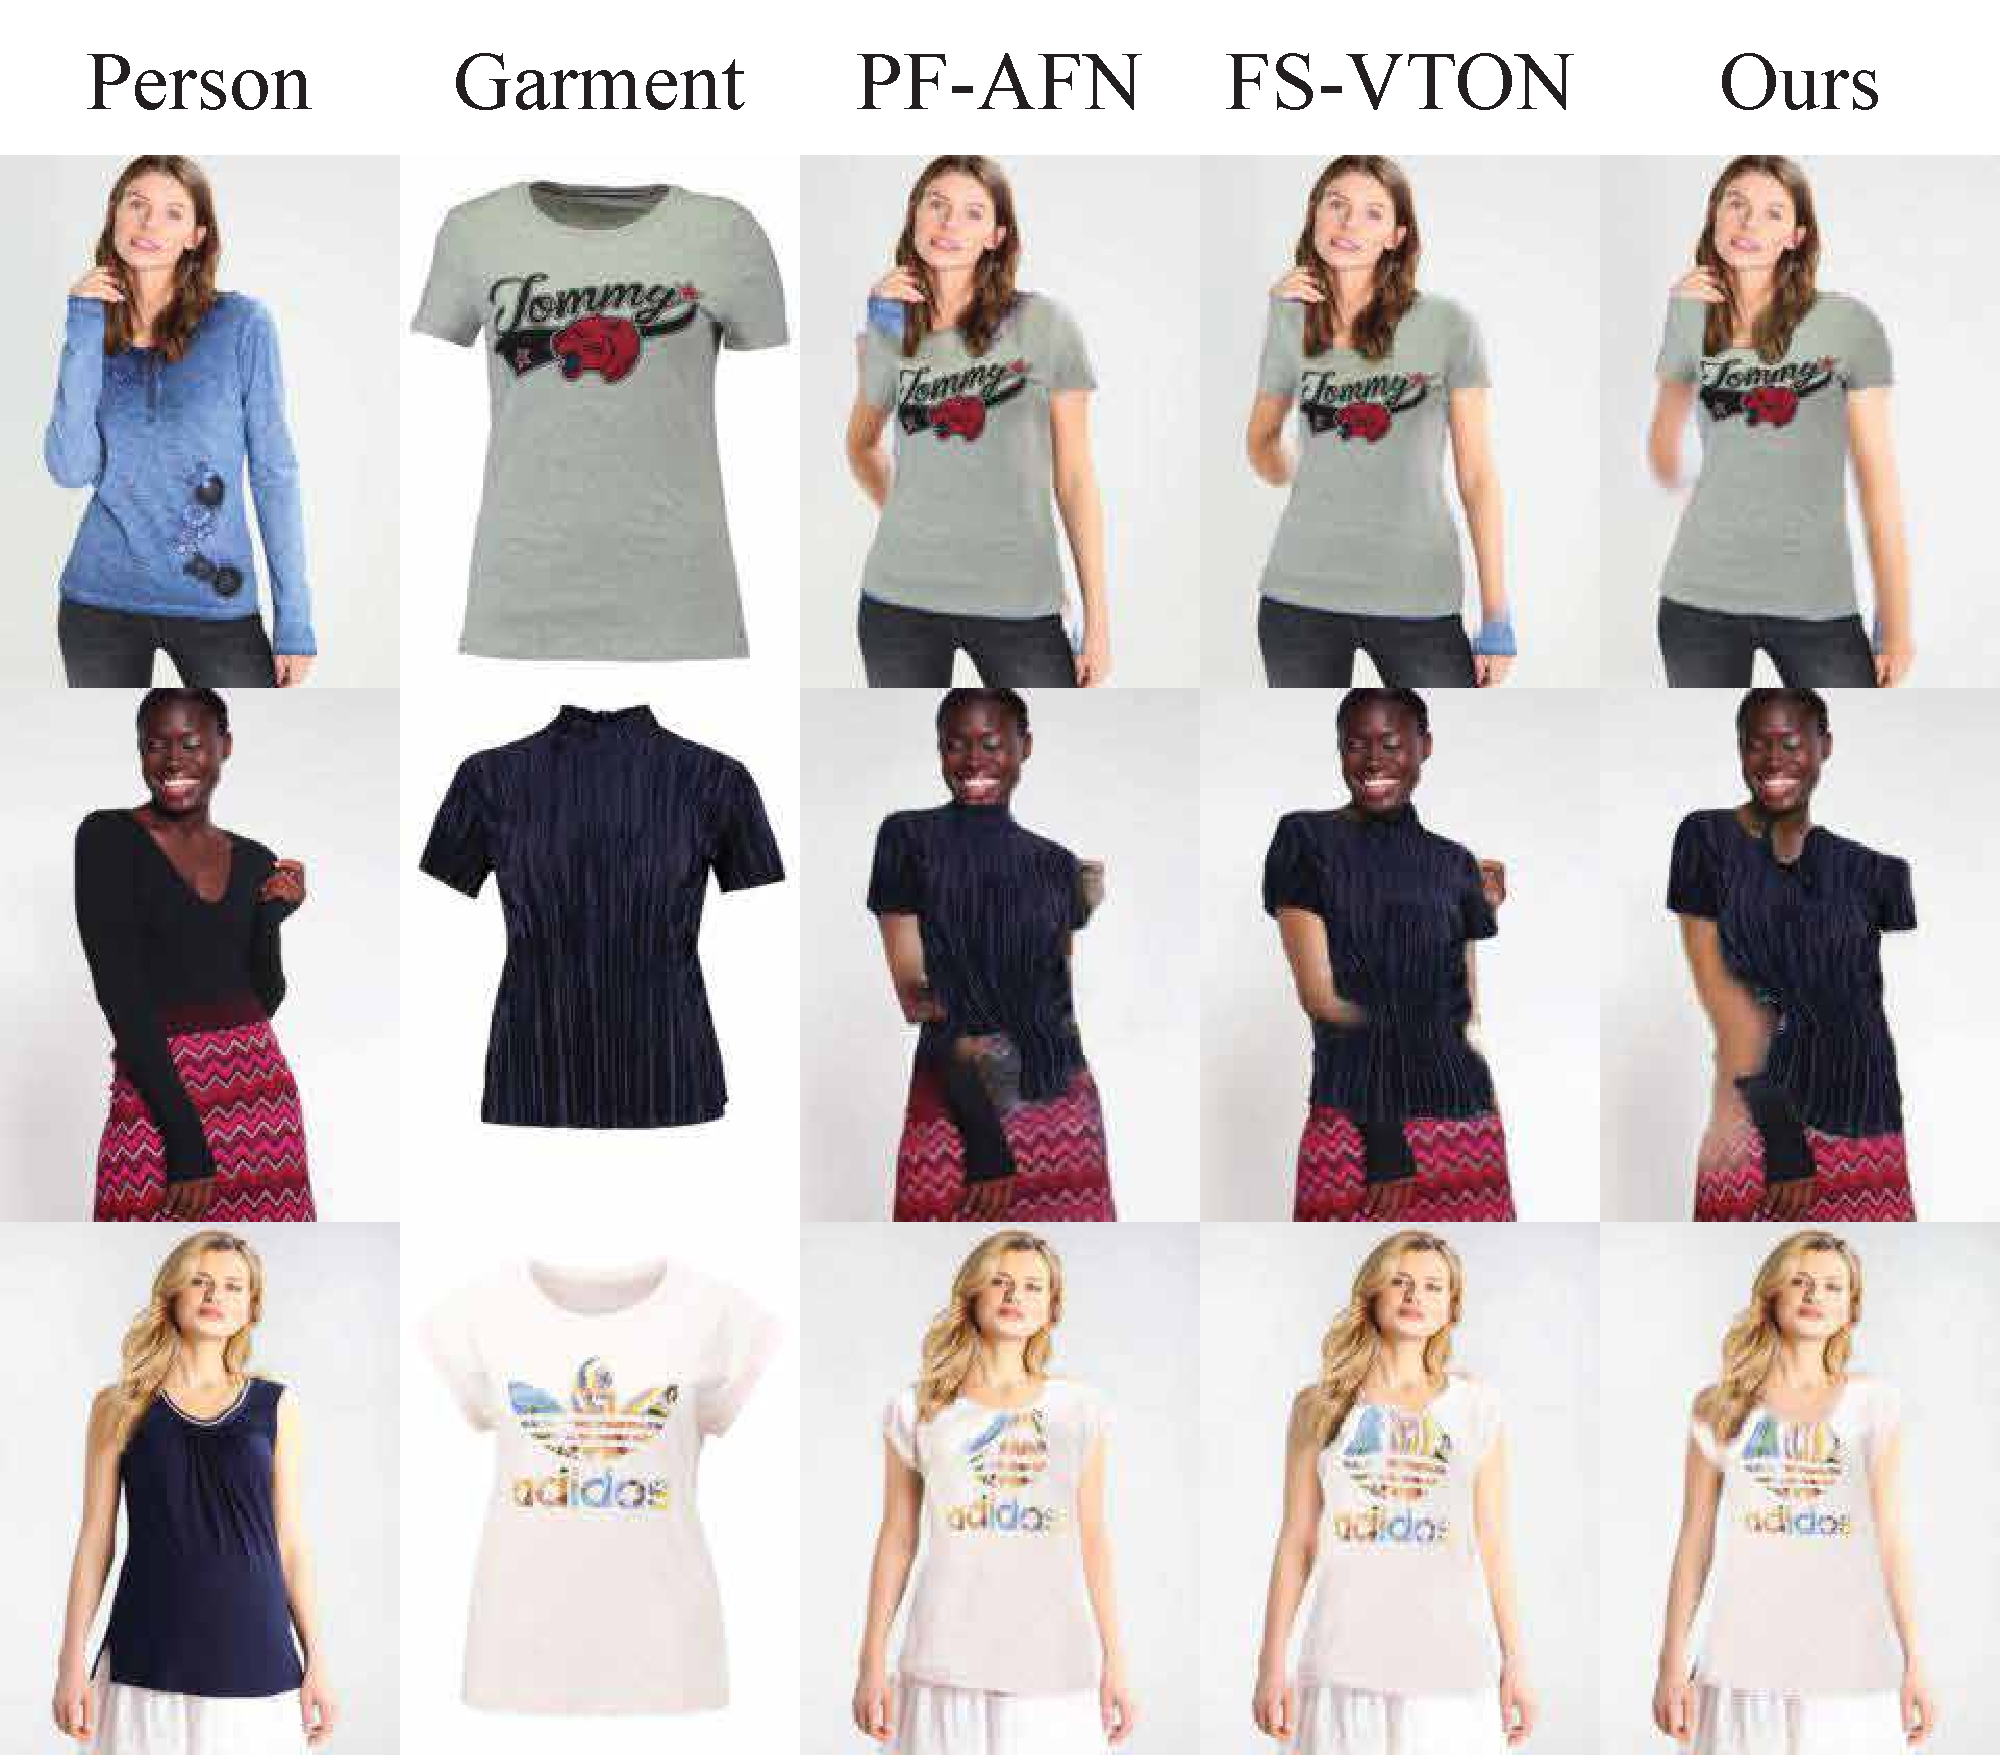
\includegraphics[width=0.7\linewidth]{content/resources/images/application/limit-cases.pdf}
    \caption{The issues of existing parser-free virtual try-on methods (i.e. PF-AFN~\cite{Ge-CVPR2021-Parser}, FS-VTON~\cite{He-CVPR2022-Style})}
    \label{fig:limit-cases}
\end{figure}

First, the try-on results are unrealistic under certain circumstances, particularly in non-straight-arm poses or when there are differences in size between the model and the clothing items.
Second, if the background color is not distinguishable from the input image, the model struggles to separate them and may blend the target garment with the background in the output image. And if the image is not captured in proper lighting conditions, the system may face difficulties in accurately reconstructing the skin area. This is because our current training dataset only includes images with clean backgrounds, with similar lighting conditions. Third, the algorithm attempts to warp the input to align with the preserved region's boundary, resulting in texture distortion.
It is important to note that similar issues have been observed in other SOTA parser-free methods (i.e. PF-AFN~\cite{Ge-CVPR2021-Parser}, FS-VTON~\cite{He-CVPR2022-Style}) also had similar problems (please refer to~\autoref{fig:limit-cases}). 

Lastly, to enhance the application's capabilities, we also aim to incorporate additional clothes categories (e.g. accessories and pants), into the try-on feature. This will lead to a more comprehensive system that allows you to receive recommendations and try on complete outfits, not just a single item.
